
\QCMautoevaluation{Pour chaque question, plusieurs réponses sont
  proposées.  Déterminer celles qui sont correctes.}

\begin{QCM}
  \begin{GroupeQCM}
    \begin{exercice}
       \begin{center} \scalebox{1}{

\begin{tikzpicture}[general]

\draw (-1,-1) node[below] {$A$};
\draw (0,-1) node[below] {$B$};
\draw (0,0) node[below right] {$C$};
\draw (-1,0) node[above] {$D$};
\draw (0,0) node[above left] {$A'$};
\draw (1,0) node[right] {$B'$};
\draw (1,1) node[above right] {$C'$};
\draw (0,1) node[above] {$D'$};

\draw[line width = 1.5pt] (-1,-1) -- (0,-1) -- (0,0) -- (-1,0) -- cycle;
\draw[line width = 1.5pt] (0,0) -- (1,0) -- (1,1) -- (0,1) -- cycle;

\end{tikzpicture}
}
 \end{center}
       Le carré $A'B'C'D'$ est l'image du carré $ABCD$ par la translation de vecteur \ldots
      \begin{ChoixQCM}{4}
      \item $\overrightarrow{AB}$
      \item $\overrightarrow{AC}$
      \item $\overrightarrow{AD}$
      \item $\overrightarrow{BD}$
      \end{ChoixQCM}
\begin{corrige}
     \reponseQCM{b}
   \end{corrige}
    \end{exercice}
    
    
    \begin{exercice}
         \begin{center} 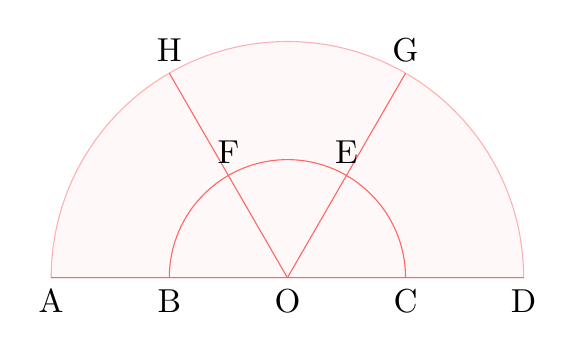
\begin{tikzpicture}	
  
    
\def \CharSize {1.2};
\def \BulletSize {1};


    %Définition de l 'angle de rotation de la figure
    \def \Rotation {0} 
    %Couleur des élèments de la figure (sauf le remplissage)
    \def \RapColor {red!60}


\begin{scope}[rotate=\Rotation]
    % contours
    \draw[color=\RapColor, fill =red!5, opacity=0.5] (-3,0) arc(180:0:3)--(3,0)--(-3,0)--cycle;	%Dont couleur de remplissage
    \draw[color=\RapColor] (-3,0)--(3,0);
    
   % demi-cercle intérieur :
    \draw[color=\RapColor](-1.5,0) arc(180:0:1.5);
    
    % rayons :
   \foreach \a in {0,60,...,180}{\draw[color=\RapColor] (\a:3)--(\a:0);}
   
 
  
\end{scope}

\draw (0,0) node [below,scale=\CharSize]{O};
\draw (1.5,0) node [below,scale=\CharSize]{C};
\draw (3,0) node [below,scale=\CharSize]{D};
\draw (-1.5,0) node [below,scale=\CharSize]{B};
\draw (-3,0) node [below,scale=\CharSize]{A};
\draw (60:1.5) node [above,scale=\CharSize]{E};
\draw (120:1.5) node [above,scale=\CharSize]{F};
\draw (60:3) node [above,scale=\CharSize]{G};
\draw (120:3) node [above,scale=\CharSize]{H};
    
\end{tikzpicture} 
  \end{center}
      $E$ est l'image de $F$ par la rotation de centre $O$ et d'angle \ldots
      \begin{ChoixQCM}{4}
      \item $+ 30^\circ$
      \item $- 30^\circ$
      \item $+ 60^\circ$
      \item $- 60^\circ$
      \end{ChoixQCM}
\begin{corrige}
     \reponseQCM{d}
   \end{corrige}
    \end{exercice}
    
    
    \begin{exercice}
      Sur l'image ci-dessus, l'image de $D$ par une rotation de centre $O$ et d'angle $120^\circ$ est \ldots
      \begin{ChoixQCM}{4}
      \item $A$
      \item $H$
      \item $G$
      \item $O$
      \end{ChoixQCM}
\begin{corrige}
     \reponseQCM{b}
   \end{corrige}
    \end{exercice}


\end{GroupeQCM}
\end{QCM}

  
